\documentclass{ctexart}

\usepackage[b5paper,scale=0.8]{geometry}
\usepackage{fontspec}
\usepackage{tcolorbox}

\usepackage{amsthm,amssymb}
\usepackage{realscripts}
\usepackage{tabu,multirow}
\usepackage{setspace}
\usepackage{caption}
\usepackage{csquotes}
\usepackage{tikz,pgfplots,tikz-cd}
\usepackage{ulem}
\usepackage{extarrows}
\usepackage[]{hyperref}
\usepackage{footnote}
\usepackage{microtype}
\usepackage{unicode-math}
\usepackage{pxrubrica}
\usepackage{fancyhdr}
\usepackage{xcolor}
\pagestyle{fancy}
\tcbuselibrary{skins, breakable, theorems, most}
\xeCJKDeclareSubCJKBlock{symbolCJK}{"2018 , "201C , "300C , "300E , "3014 , "FF08 , "FF3B , "FF5B ,"3008 , "300A , "3016 , "3010 , "2026 , "3001 , "3002 , "FF0C , "FF0E , "FF1A , "FF1B ,"FF01 ,"FF1F , "FF05 , "3015 , "FF09 , "FF3D , "FF5D , "3009 ,"300B , "3017 , "3011 , "2019 , "201D , "300D , "300F}
\xeCJKDeclareSubCJKBlock{symbolCJKpozhe}{"2014}

\setCJKmainfont[symbolCJK=EB Garamond,symbolCJKpozhe=方正纤雅宋简体,BoldFont=GenYoMin TW B]{GenWanMin TW TTF}
\newCJKfontfamily{\sansgsgtw}{GenSekiGothic TW}
\newtcbtheorem[number within=section]{tho}{定理}%
  {colback=gray!5,colframe=gray!35!black,fonttitle=\bfseries,arc=0mm}{th}

\setmathfont{Garamond-Math.otf}[StylisticSet={2, 7, 9}]
\setmathfont{Garamond-Math.otf}[StylisticSet={2, 7, 9, 8}, version=a]
\renewcommand{\symcal}[1]{{\mathversion{a}\mbox{$\symscr{#1}$}}}
\newcommand{\dx}{\symscr{D} _t (x)}

\defaultfontfeatures{%
RawFeature={
	+calt,+swsh,+liga,+hlig,+clig,+dlig,+cv01}
  }

\setmainfont{EBGaramond12-Regular.otf}[ItalicFont = EBGaramond12-Italic.otf]%[Ligatures = Rare,Ligatures = Historic,Style=Historic]
\setmathfont[range = "0211C]{Latin Modern Math}
\everymath{\displaystyle}

\renewcommand{\textbf}[1]{\mbox{\bfseries#1}}
\catcode`\,=13
\def,{\kern0.05em,\kern0.45em}
\catcode`\。=13
\def。{\kern0.05em.\kern0.45em}
\catcode`\:=13
\def:{:\kern0.5em}
\catcode`\;=13
\def;{;}
\catcode`\!=13
\def!{!}
\catcode`\?=13
\def?{\,?\kern0.5em}
\catcode`\(=13
\def({\raisebox{0.28ex}{\,(}}
\catcode`\)=13
\def){\raisebox{0.28ex}{)\,}}
\catcode`\“=13
\def“{``}
\catcode`\”=13
\def”{''}


\begin{document}
\setcounter{section}{-1}

\section*{前言}

这篇文章(如果写得完的话)应该是一篇 ODE 的小短文,按照笔者的想法,笔者更倾向于将叙述形式变为两个人之间的对话,这两个人就叫做“朱鹭子”和“琪露诺”吧(笑),至于为什么……那只是因为笔者喜欢罢了(笑)。

由于笔者才疏学浅,其中必定错漏百出,请多指教。

\rightline{\ruby[g]{小飞舞}{Innocent\ FIVE}}
\newpage
\tableofcontents
\newpage
\phantom{2}
\vspace{2em}
\begin{spacing}{2}
	\thispagestyle{empty}
	\rightline{\Huge\parbox{1em}{\fontsize{60pt}{80pt}{\bfseries 朱鹭子和琪露诺}}\hspace{2em}}
\end{spacing}
\clearpage
\section{什么是ODE}
朱鹭子:ODE被称为“常微分方程”,是一种奇怪的方程,它代表了一些奇怪的量之间的奇怪关系,我记得你是学过微积分的吧?

琪露诺:呃……学过一点(挠头)。

朱鹭子:那就好,线性代数呢?

琪露诺:emmmm…… 只看过那本同济的……

朱鹭子:我的天……那本啊……算了也没关系,都一样的……行,那我开始说了啊……
\section{一阶ODE的初等解法}
朱鹭子:一阶的ODE在某种意义上是最简单的ODE了,所以我们可以先来研究它。我们知道,ODE事关待求解函数 \(x(t)\) 的导数,这个导数可能是很高阶的,比如:

\[
	\symscr{D} ^n_t (x)=f(t,x)
	.\]

此时我们……

琪露诺:等等等等,这个 \(\symscr{D} \) 是什么……

朱鹭子:哦这个啊,我们管它叫“求导算符”,这里这样写指的是对 \( t\) 求 \(n\)次导,同时,我们也默认 \(x\) 是关于 \(t\) 的函数。我么继续,上面这个式子是一个 \(n\)阶的ODE,我们不想讨论它,我们直接来看最简单的:
\[
	\symscr{D} _t (x)=f(t)g(x)
	.\]
这种被称为“变量分离方程”。
\subsection{变量分离方程}
朱鹭子:这种我们可以这样做:
\[
	\frac{\symscr{D} _t(x)}{g(x)}= f(t)
	.\]
两边积分就可以得到:
\[
	\int \frac{1}{g(x)} \,\mathrm{d}x =\int f(t) \,\mathrm{d}t \tag{A}
	.\]

琪露诺:诶等等,这个 \(\symscr{D} _t(x)\) 到哪里去了?

朱鹭子:啊这个的话……实际上是有
\[
	\int \frac{1}{g(x)} \,\mathrm{d}x =\int \frac{\symscr{D} _t(x)}{g(x)} \,\mathrm{d}t
	.\]
这个,这个你不是有学的吗?

琪露诺:呃我忘了……

朱鹭子:啊这……好,现在我们看 A 方程的两边,左边只和 \(x\) 有关,右边只和 \(t\)有关,那么我们实际上就把 \(x(t)\)解出来了,虽然用的是隐式方程的表示法。

琪露诺:原来如此,这有什么要注意的地方吗?

朱鹭子:有,积分记得加上常数。接下来我们来看另外一种方程。
\subsection{线性微分方程}
朱鹭子:好,我们来看看这种:
\[
	\dx{}+p(t)x=f(t)\tag{B}
	.\]
这种被称为线性微分方程。

琪露诺:诶……这个线性指的是什么意思呢……

朱鹭子:我们可以这样理解。假设 \(x_1\)和 \(x_2\)都是方程  B 的解,那么我们考虑:
\[
	x_3=cx_1+(1-c)x_2
	.\]
这个是不是方程B的解呢?

琪露诺:emmmm好像是的。

朱鹭子:对,没错,这里实际上是有:
\[
	\begin{cases}
		\\[-2.2em]\
		\symscr{D} _t^n(x_1+x_2)=\symscr{D} _t^n(x_1)+\symscr{D} _t^n(x_2), \\
		\symscr{D} _t^n(cx_1)=c\cdot \symscr{D} _t^n(x_1).
	\end{cases}\tag{C}
\]
这里指的是求导算符的函数线性,另外我们考虑更普遍的形式:
\[
	\begin{aligned}
		 & \symscr{L}_1 =\symscr{D} _t^n +a_{n-1}(t)\symscr{D} _t^{n-1}+\cdots a_1(t)\symscr{D} _t +a_0(t)=\symscr{D} _t^{n-1}+\sum\limits_{i=1}^{n-1} a_{i}(t)\symscr{D} _t^i , \\
		 & \symscr{L}_2 =\symscr{D} _t^n +b_{n-1}(t)\symscr{D} _t^{n-1}+\cdots b_1(t)\symscr{D} _t +b_0(t)=\symscr{D} _t^{n-1}+\sum\limits_{i=1}^{n-1} b_{i}(t)\symscr{D} _t^i.
	\end{aligned}
\]
那么算符 \(\symscr{L}_1 \)和 \(\symscr{L} _2\)满足:
\[
	\left(\symscr{L} _1+\symscr{L} _2 \right) (x)=\symscr{L} _1(x)+\symscr{L} _2 (x)
	.\]
这被称为算符线性。

因此合并起来就是:

\[
	\left( \symscr{L} _1+\symscr{L} _2 \right) \left( x_1+x_2 \right) =\symscr{L} _1(x_1)+\symscr{L} _1(x_2)+\symscr{L} _2(x_1)+\symscr{L} _2(x_2)
	.\]

琪露诺:哦哦,原来线性指的是我可以随意拆掉括号啊……

朱鹭子:不可以哦,只是满足C方程罢了,你只能在规定的范围内行动。虽说如此,线性方程确实是比较简单的一类。好,我们来看B方程,这个怎么解呢?

琪露诺:我在寺子屋里见过这些题,一般来说左边都是一些函数的导数,然后两边积分就可以求出函数出来。

朱鹭子:没错,但是在这里,这个 \(p(x)\) 是如此随机,左边很可能不是个新函数的导数,我们应该怎么办呢?

琪露诺:emmmm呜哇哇……

朱鹭子:事实上,我们可以乘上一个新的函数,改变左边那一坨的结构:
\[
	B \implies h(t)\dx{}+h(t)p(t)x=f(t)h(t)\tag{D}
	.\]

琪露诺:可是这样左边还是很怪啊,看起来根本不像个导数……

朱鹭子:是的,所以我们硬来,考虑新的函数 \(h(t)x\),那么它的导数就是:
\[
	\symscr{D} _t\left( h(t) x(t)  \right)= h(t) \dx +\symscr{D} _t(h(t))x
	.\]
这样我们观察D式,我们可以强行要求:
\[
	h(t)p(t)=\symscr{D} _t\left( h(t) \right)
	.\]

琪露诺:看起来像那个巫女的作风……

朱鹭子:不是哦,\sout{灵梦哪有那么聪明}。好了,接下来我们的任务就是解出这个奇怪的 \(h(t)\),还记得变量分离方程吗?\(h(t)\)的约束就是这个变量分离方程哦。

琪露诺:记得,所以我们只要:
\[
	h(t)p(t)=\symscr{D} _t\left( h(t) \right) \implies \int \frac{1}{h(t)} \,\mathrm{d}h =\int p(t) \,\mathrm{d}t
	.\]

这意味着:

\[
	\ln h(t)= \int p(t) \,\mathrm{d}t \implies h(t)=\symrm{e} ^{\int p(t) \,\mathrm{d}t }
	.\]

朱鹭子:不对哦,你积分没加常数。

琪露诺:呜哇……那加了常数之后,就是:
\[
	\ln h(t)= \int p(t) \,\mathrm{d}t +c_1\implies h(t)=\symrm{e} ^{c_1}\cdot \symrm{e} ^{\int p(t) \,\mathrm{d}t }
	.\]

是这样吗?

朱鹭子:其实你可以不加的,因为你有一个积分号没有被消掉……但先不管这个,我们可以看到 \(h\)我们已经求出来了,接下来呢?

琪露诺:那这个  \(c_1\)怎么确定啊?

朱鹭子:不用确定,都是满足条件的不是吗?为了容易算我们就让它是0好了。

琪露诺:哦哦,那这样子C方程就是:
\[
	\symscr{D} _t(h(t)x)=f(t)h(t)
	.\]

这是一个变量分离方程,我可以对它进行积分:
\[
	h(t)x= \int f(t)h(t) \,\mathrm{d}t \implies x= \frac{\displaystyle \int f(t)h(t) \,\mathrm{d}t}{h(t)}
	.\]

最后是代入 \(h(t)\)的方程得到:
\[
	x=\frac{\displaystyle \int f(t)\symrm{e} ^{\int p(t) \,\mathrm{d}t } \,\mathrm{d}t}{\symrm{e} ^{\int p(t) \,\mathrm{d}t }}
	.\]

哇,这啥啊……

朱鹭子:你做的是正确的,这就是B方程的解啦。

\subsection{常数变易法}

琪露诺:原来如此,所以这一节我完全懂了对吧。

朱鹭子:不是哦,再和你说些东西,我们回过头考虑一种更简单的情况:
\[
	\dx+p(t)x=0
	.\]

琪露诺:我知道我知道,这是分离变量方程!

朱鹭子:对,他的解是 \(x=c_1\exp \left(- \int p(t) \,\mathrm{d}t  \right) \) ,我们反倒可以这样考虑,这个 \(c_1\) 并不是一个常数,而是一个函数 \(c_1(t)\),此时 \(x=c_1(t)\exp \left(- \int p(t) \,\mathrm{d}t  \right)\)反倒是方程B的解,那么会发生什么事呢?

琪露诺:我猜猜……将这个新东西带进去之后会得到一个新的方程。

朱鹭子:没错,我们试试看:
\[
	\begin{aligned}
		 & \phantom{=}\ \,\,\dx+p(t)x={\color{brown}\symscr{D} _t\left( c_1(t)\exp \left(- \int p(t) \,\mathrm{d}t  \right) \right)} +p(t) c_1(t)\exp \left(- \int p(t) \,\mathrm{d}t  \right)
		\\
		 & ={\color{brown}\symscr{D} _t(c_1(t))\exp \left(- \int p(t) \,\mathrm{d}t  \right)+c_1(t)\exp \left(- \int p(t) \,\mathrm{d}t  \right)(-p(t))}+p(t) c_1(t)\exp \left(- \int p(t) \,\mathrm{d}t  \right) \\
		 & = \symscr{D} _t(c_1(t))\exp \left(- \int p(t) \,\mathrm{d}t  \right) =f(t).
	\end{aligned}
\]

琪露诺:所以这个 \(c_1(t)\)就满足:
\[
	c_1'(t)=f(t)\exp \left(\int p(t) \,\mathrm{d}t  \right) \implies c_1(t)=\int \left[ f(t)\exp \left(\int p(t) \,\mathrm{d}t  \right)  \right]  \,\mathrm{d}t
	.\]

天……这太多积分号了叭……

朱鹭子:确实,但这玩意不是和你之前求的B方程的解差不多吗?

琪露诺:哦也是,那这个方法有什么用呢?

朱鹭子:用处多了,以后我们在解更普遍的方程会用到这个解法,这被称为\textbf{常数变易法}。

琪露诺:哦……

朱鹭子:接下来我们看些更神奇的。

\subsection{恰当微分方程}
考虑一些更通用的情况:
\[
	\dx=f(x,t)
	.\]

我们可以把它写成微分形式:

\[
	f(x,t)\,\symrm{d} t-\symrm{d} x=0
	.\]

再考虑更一般的情况:

\[
	T(x,t)\,\symrm{d} t+ X(x,t)\,\symrm{d} x=0
	.\]

琪露诺:这是啥……

朱鹭子:看到了吗?这其实是微分方程的一种特殊写法,看到这你想到了什么?

琪露诺:emmm……第二类线积分?

朱鹭子:没错!第二类线积分里面有些很好算的情况,那就是“路径无关”的时候,此时应该由什么判别呢?

琪露诺:emmm由Green公式应该有:

\[
	\frac{\partial T}{\partial x}=\frac{\partial X}{\partial t}
	.\]

朱鹭子:在函数性质良好的前提下,可以这么做,那么如果是路径无关的话接下来这么求解方程呢?

琪露诺:呃……

朱鹭子:事实上,路径无关场就是梯度场,这意味着存在一个函数 \(u\) 使得:
\[
	\frac{\partial u}{\partial t}=T,\qquad \frac{\partial u}{\partial x}=X
	.\]
所以方程就变成了:
\[
	\frac{\partial u}{\partial t}\,\symrm{d} t+ \frac{\partial u}{\partial x}\,\symrm{d} x=0
	.\]

左边就是 \(u\)的全微分啦,所以我们就有:

\[
	u=c_1
	.\]

这样就解出了 \(x\)了。

琪露诺:那如果没有路径无关怎么办?

朱鹭子:你可以想一下,我们之前怎么解决不是全微分的问题的。

琪露诺:emmm难道你说的是,乘上一个新的函数?

朱鹭子:可以这样做,看看吧:
\[
	\frac{\partial u}{\partial t}=hT,\qquad \frac{\partial u}{\partial x}=hX
	.\]

接下来呢?

琪露诺:呃……不知道了。

朱鹭子:事实上我们可以考虑Young定理:
\[
	\frac{\partial ^2u}{\partial x \partial t}=\frac{\partial ^2u}{\partial t \partial u}\implies \frac{\partial (hT)}{\partial x}=\frac{\partial (hX)}{\partial t}
	.\]

接下来我们可以用乘法法则分离它们:
\[
	X \frac{\partial h}{\partial t}-T \frac{\partial h}{\partial x}=\left( \frac{\partial T}{\partial x}-\frac{\partial X}{\partial t} \right) h
	.\]

琪露诺:好的,那这个方程怎么解?

朱鹭子:事实上这是一个偏微分方程……单纯解它比解原来的ODE更困难。

琪露诺:啊这……这不就是……寄了吗?

朱鹭子:差不多吧,不过的确有一些比较简单的情况。

\begin{itemize}
	\item 当 \( \frac{\frac{\partial T}{\partial x}-\frac{\partial X}{\partial t}}{X} =p(t)\) 与 \(x\) 无关的时候。我们有:
	      \[
		      h(t,x)=\exp \left( \int p(t)\,\mathrm{d}t  \right)
		      .\]
	\item 当 \( \frac{\frac{\partial T}{\partial x}-\frac{\partial X}{\partial t}}{T} =q(x)\) 与 \(t\) 无关的时候。我们有:
	      \[
		      h(t,x)=\exp \left(- \int q(x)\,\mathrm{d}x \right)
		      .\]
	\item 当 \( {\frac{\partial T}{\partial x}-\frac{\partial X}{\partial t}}=p(t)X-q(x)T\)的时候。我们有:
	      \[
		      h(t,x)=c_1 \exp \left( \int p(t) \,\mathrm{d}t +\int q(x) \,\mathrm{d}x  \right)
		      .\]
\end{itemize}

琪露诺:前两个还好,第三个也太那啥了,这个只有天才才能看出来吧。

朱鹭子:这个不管,反正算是比较简单的情况了(笑)。当然你也可以直接用看就把这个 \(h\)(我们管它叫积分因子)找出来。

琪露诺:这能看出来的吗?

朱鹭子:看你的直觉了……比如说这个?
\[
	\left( x^2 +y^2 +x \right) \,\symrm{d} x +y \,\symrm{d} y=0
	.\]

琪露诺:哇……看起来好难……哭……

朱鹭子:看,其实我们仔细观察的话倒是可以看出一些对偶量:
\[
	\left( x^2 +y^2  \right) \,\symrm{d} x +y \,\symrm{d} y+ x \,\symrm{d} x=0
	.\]

尝试 \(h=\frac{1}{x^2 +y^2 }\),我们可以得到:
\[
	\symrm{d} x+ \frac{x\,\symrm{d} x+y\,\symrm{d} y}{x^2 +y^2 }=0\implies \symrm{d} x+\symrm{d} \left( \frac{1}{2}\ln \left( x^2 +y^2  \right)  \right) =0
	.\]

所以最后的结果就是:
\[
	x+ \frac{1}{2}\ln \left( x^2 +y^2  \right)=c_1
	.\]

琪露诺:这根本不是人能看出来的……

朱鹭子:诶别说,这种对那只九尾策士的确是显然的题……

琪露诺:啊。所以,一阶微分方程就到这里了?

朱鹭子:不对哦,这只是一些基础的,还有一些奇怪的情况需要提及一下。那就是其解的参数表示。

琪露诺:emmm好像确实之前没有讲关于参数方程的任何内容呢……

朱鹭子:我们来看一些隐式方程:
\[
	x=f(t,x')
	.\]

这种反倒是将 \(x\) 分离出来了,此时怎么办呢?

琪露诺:emmm这不又是一个一般的式子吗,怎么可能会有什么通法?

朱鹭子:你想想看吧,这种和之前的有什么不同?

琪露诺:emmm首先是 \(x'\)不能再随意地被分离出来,然后是左边是 \(x\)……

朱鹭子:差不多,想想左边有没有办法变成 \(x'\)呢?

琪露诺:啊,你是说求导?

朱鹭子:对咯:

\[
	\dx= \frac{\partial f}{\partial t}+ \frac{\partial f}{\partial \left( x' \right) }\symscr{D} _t^2(x)
	.\]

我们不妨设 \(p= \dx\),那么这个方程就可以变为:

\[
	p=\frac{\partial f}{\partial t}+ \frac{\partial f}{\partial p}\symscr{D} _t(p)
	.\]

琪露诺:可是这个方程不还是很怪吗?也不是有通解的那种……诶等等,这下好像 \(\symscr{D} _t(p)\)就分离出来了:
\[
	\symscr{D} _t(p)= \frac{p-{\partial f}/{\partial t}}{{\partial f}/{\partial p}}
	.\]

接下来我只要按照前面三种方法做就可以解出 \(p\),然后积分就可以得到 \(x\)了对吧?

朱鹭子:差不多是这样,但是如果你解出来 \(p\),但是却是无法分离的,导致你没法直接积分,那该怎么办呢?况且你既然能解出 \(p\),把它往 \(f\)里面一代,不就把 \(x\)解出来了吗,为什么要积分呢?

琪露诺:啊啊啊哇。

朱鹭子:最令人难受的应该是你解出来得到这个吧:

\[
	\psi (t,p,c_1)=0
	.\]

你看,你甚至连通解的参数都是嵌在函数里面的,此时你不考虑参数方程还能怎么办呢?

琪露诺:通解参数是什么哇?

朱鹭子:啊,就里面这个 \(c_1\),事实上对于一个 \(n\)阶的微分方程,它的通解将会长得像:
\[
	x=\psi (t,c_1,c_2,\cdots ,c_n)
	.\]

其中 \(c_1,c_2,\cdots ,c_n\) 相互独立,这到时候说一下唯一性定理你可能会更明白一些。

琪露诺:好吧,所以最后的参数方程就是:
\[
	\begin{cases}
		\\[-2.2em]\
		\psi (t,p,c_1)=0, \\
		x=f(t,p).
	\end{cases}
\]

这样咯?那参数就是那个 \(t\)咯。

朱鹭子:\(t\)是自变量,\(p\)才是参数。你要知道 \(p\)才是我们想要消去的那个,所以 \(p\)是参数。

琪露诺:哦。所以这其实是一种“差不多解出来了但还有一步要走”的情况吧?

朱鹭子:的确,看看这种?
\[
	t=f(x,x')
	.\]

这下反倒是自变量被分离出来了。

琪露诺:麻……这是强行走成反函数的路线吗……

朱鹭子:要清楚你现在考虑的是微分结构,不要乱反函数。

琪露诺:呜……首先我左右两边对 \(t\)求导:
\[
	1=\frac{\partial f}{\partial x}\symscr{D} _t(x)+ \frac{\partial f}{\partial (x')}\symscr{D} _t^2(x)
	.\]

然后再设 \(p=\symscr{D} _t(x)\) ,这样子就行啦:
\[
	1=\frac{\partial f}{\partial x}p+ \frac{\partial f}{\partial p}\symscr{D} _t(p)
	.\]

朱鹭子:不错,这也有另外一种方法,那就是上来直接对 \(x\)求导:
\[
	\symscr{D} _x(t)=\frac{\partial f}{\partial x}+\frac{\partial f}{\partial p}\symscr{D} _x(p)
	.\]

然后由于一阶微分形式的不变性,我们可以把它改写为:
\[
	\frac{1}{p}=\frac{\partial f}{\partial x}+\frac{1}{p}\cdot \frac{\partial f}{\partial p}\symscr{D} _t(p)
	.\]

也和你写的一样哦。

琪露诺:哇塞。

朱鹭子:嗯,来点更怪的例子,如果你最后解出来是这样子的:

\[
	\begin{cases}
		\\[-2.2em]\
		x'=X(c) , \\
		\ t=T(c).
	\end{cases}
\]

这种情况呢?你该怎么得到——没有其他条件了—— 那个\(x\)呢?

琪露诺:寄。我试试看,首先是:
\[
	\symscr{D} _c(x)=\symscr{D} _t(x)\symscr{D} _c(t)= X(c)T'(c)\implies \begin{cases}
		\\[-2.2em]\
		x=\int   X(c)T'(c)\,\mathrm{d}c, \\
		\ t=T(c).
	\end{cases}
\]

依据微分形式不变性好像是这样的?

朱鹭子:的确。总而言之,你就得构造这个 \(\symscr{D} _c(x)\)然后对其积分,虽然得到的结果是参数方程,不过也值了不是吗?

琪露诺:听起来是这样没错啦……
\section{存在唯一性定理}


朱鹭子:在此之前,我们得到的ODE全都无视了它是否有没有解,\textbf{解是否唯一},这里倒是准备和你说一下这些。

琪露诺:存在性吗……感觉很枯燥……

\begin{tho}[label=czwy]{存在唯一性定理}{}
	对于一个将导数分离出来的ODE:
	\[
		\dx=f(t,x)
		.\]
	如果 \(f\)在开区域 \(\overline{\symcal{I} }\) 上面满足:任意 \(\overline{\symcal{I} }\)中的闭矩形区域 \(\overline{\symcal{G}} \)上都满足Lipschitz条件:
	\[
		\left\vert f(t,x_1)-f(t,x_2) \right\vert \leqslant L \left\vert x_1-x_2 \right\vert ,\,\forall (t,x_1),(t,x_2)\in \overline{\symcal{G}}
		.\]

	且有初始条件:\(x(t_0)=x_0\),则存在解 \(x=X(t) \)在点 \((t_0,x_0)\)的邻域内有定义,且该解可以延拓到任意接近 \(\overline{\symcal{I} }\)的边界。
\end{tho}

琪露诺:???????这都啥啊……

朱鹭子:这确实很怪……让我尝试说明一下。为了方便,我们先从单变量的实函数开始说明:
\[
	y=f(x) \,\mbox{或者}\, f: \overline{\symcal{I} } \subseteq\symbb{R}     \mapsto  \symbb{R}
	.\]
如果存在常数 \(L\)使得:
\[
	\left\vert f(a)-f(b) \right\vert \leqslant L \left\vert a-b \right\vert, \,\forall a,b\in  \overline{\symcal{I} }
	.\]

则我们称 \(f\)满足Lipschitz 条件,而 \(L_{\rm min}\)被称为Lipschitz常数,如果这个常数小于一,我们会称 \(f\)是\textbf{压缩映射}。这个我们先不管了,你只要先知道,如果 \(f\) 是在区域内满足Lipschitz条件,那么给出 \(x\)的一个初值条件时候,\(x\)唯一可解。

另外一件事是,要确立一个函数的Lipschitz条件是非常麻烦的一件事,我们可以用:\(\frac{\partial f}{\partial x}
\)连续来替代。

琪露诺:看起来要好不少……至少有比较良好的方式了。

朱鹭子:对,现在你可以考虑以下这种,如果你没法把 \(x'\)分离出来怎么办?
\[
	F(x,x',t)=0
	.\]
这种呢?

琪露诺:啊……我感觉……可以试试隐函数存在定理,只要在邻域内 \(\frac{\partial F}{\partial x'}\Bigg|_{(t_0,x_0)}\neq 0\)的话,那我就可以在这里把 \(x'\) 解出来。

朱鹭子:没错,这意味着有一些\(\frac{\partial F}{\partial x'}\Bigg|_{(t_0,x_0)}=0\)的情况。
\subsection{包络线}

琪露诺:什么情况呢?

朱鹭子:我和你说个问题,如果有这样一种解,它的并不属于通解,但它也是微分方程的解,而且满足一种特殊的性质:
\begin{itemize}
	\item 这条曲线的每一点处都有一条通解曲线与其相切。
\end{itemize}
这种曲线被称为上述通解积分曲线族的\textbf{包络}。

琪露诺:包络?那是什么?

朱鹭子:在这里我可以给出一些例子:

\begin{center}
	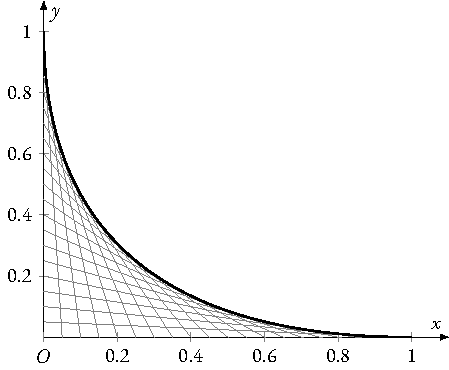
\includegraphics{envelope.pdf}
\end{center}

假如有这样一些直线,它的 \(y\)轴截距和 \(x\)轴截距加起来是 1,并且那两个截距都大于零,图中画出了一些这样的直线(灰色部分),那么黑色曲线就是它的包络线。

琪露诺:哇,好像它就是把灰色线的运动紧紧包裹住了一样。

朱鹭子:差不多,不过实际上应该是相切吧(笑),比如离原点距离为1的直线的包络就是单位圆嘛。

琪露诺:那包络线怎么求呢?

朱鹭子:实际上我们知道那些通解,或者更广泛地,曲线族的形式可以表示为:
\[
	F(t,x,c_1)=0
	.\]

那么包络线的方程是会满足:
\[
	\begin{cases}
		\\[-2.2em]\
		F(t,x,c_1) =0, \\
		\frac{\partial F}{\partial c_1}=0.
	\end{cases}\tag{E}
\]

针对 \(c_1\)的参数方程。但是满足这方程的曲线可能有很多,其中并不一定有包络线。但毫无疑问的是,包络线的确是一种特殊的存在。现在我们来看看包络线和微分方程的关系:

想想看,对于一个一阶微分方程,它对解曲线的性质描述只精确到一阶导数,那么看看我们的包络线——每一点都有一条曲线族中的曲线\textbf{与之相切},如果这族曲线是一个一阶ODE的解的话……

琪露诺:那是不是意味着,这个包络上面所有点都满足那个方程……因为导数一样了,点也在那些解的曲线上面。

朱鹭子:没错!这其实就是说这个包络线也是ODE的解,这其实是ODE的\textbf{奇解}。当然这也就意味着不满足那个唯一性条件了,所以根据你之前说的……

琪露诺:隐函数存在定理。

朱鹭子:对,所以对于初始条件 \(x(t_0)=x_0\),应当有:
\[
	\frac{\partial F(t,x,x')}{\partial x'}\Bigg|_{(t_0,x_0)}
	.\]

但这只是最基本的条件,事实上,由E式子我们知道,我们把 \(\dx\) 看成是 \(c_1\)……然后实际上这个\ruby[g]{包络}{奇解}应该满足:
\[
	\begin{cases}
		\\[-2.2em]\
		F(t,x,x')=0 \\
		\ \frac{\partial F}{\partial x'}=0
	\end{cases}
	.\]

将这玩意把 \(x'\)消去就是包络线要满足的方程了,同理,这只是其中一个条件而已。

琪露诺:又来……全都是仅仅能满足的程度吗?有没有充要条件呢?

朱鹭子:饶了我吧,我暂时还不知道(笑),上面这个主要是来判断一个ODE有没有奇解的,这样的解往往会……就像幻想乡对于外界一样吧(笑)。

琪露诺:又是听不懂的比喻……

朱鹭子:这倒是有个出名的例子,叫做Clairaut微分方程:
\[
	x=t\symscr{D} ^2_t(x)+f\left( \dx\tag{ſ} \right) \symscr{D} ^2_t(x)
	.\]

琪露诺:这是什么奇怪的记号……积分号吗?

朱鹭子:这个不管,你试试鼓捣鼓捣这个ODE。

琪露诺:哦……首先两边对 \(t\)求导,得到:
\[
	\dx=x\symscr{D} ^2_t(x)+\dx+f'\left( \dx \right)\symscr{D} ^2_t(x)
	.\]

约去两边的 \(\dx\)得到:
\[
	\symscr{D} ^2_t(x)\left( x+f'\left( \dx \right)  \right) =0
	.\]

所以事实上是 \(\symscr{D} ^2_t(x)=0\implies \dx=c_1\)和 \(x+f'\left( \dx \right)=0 \)。

接下来我只需要积分就可以……哦直接代方程……就可以:
\[
	x=c_1x+f(c_1)
	.\]

哇是一坨子直线。所以你的意思是说另外一个 \(x+f'\left( \dx \right)=0\)其实是这些直线的包络吗?

朱鹭子:事实上的确是这样,在这里就先不验证了,但不管怎么样,记住有奇解存在这件事还是相当重要的。


\newpage
\phantom{2}
\vspace{2em}
\begin{spacing}{2}
	\thispagestyle{empty}
	\rightline{\Huge\parbox{1em}{\fontsize{60pt}{80pt}{\bfseries 八云蓝和橙}}\hspace{2em}}
\end{spacing}
\clearpage
\section{一阶微分方程的简单换元法}

橙:蓝大人,这道题怎么做啊:
\[
	\dx = \frac{t^2 +x^2 +tx}{tx}
	.\]

求它的通积分。

蓝:显然是 \(\ln(x+t)-\frac{x}{t}=c_1 \)(笑)。




\clearpage
\textit{Paradise Loſt}

sucking(\textit{sucking})

ſucking(\textit{ſucking})

fucking(\textit{fucking})
ſsf(\textit{ſsf})
\[
	\sum\limits_{n=1}^{\infty} \frac{1}{n^{s}}=\zeta(s),\,\mathrm{when}\ \Re(s)>1
	.\]

\[
	\varepsilon
	.\]
Paradise Lost

I can eat glass, it can't hurt me.
\end{document}